\chapter{GUI Builder Service Specification}
\section*{\textit{Version 1.0}}
\section{Introduction}

The GUI Builder Service provides a user-interface-agnostic solution to create UIs
for simple user input. The UIs are built from the user interface specification
provided by \class{MetaTypeProvider} and requires no UI coding to be done other
than providing an implementation of \class{MetaTypeProvider}. Information on
creating these classes can be found in section \ref{GUISpec}. In addition, simple
methods for creating warnings, pop-ups, and simple yes/no dialog boxes are
provided by the GUI Builder Service. The GUI creation workflow is illustrated in
figure \ref{fig:guiCreationWorkflow}.

\subsection{Entities}

\begin{itemize}
  \item \textit{GUIBuilderService} - The Service interface for creating
  user interfaces and dialog boxes.
  \item \textit{MetaTypeProvider} - The interface for creating simple user
  interface specifications.
  \item \textit{GUI} - The interface for controlling the
  \class{GUIBuilderService} generated user interface.
  \item \textit{SelectionListener} - The interface to listen for events
  generated by the user's interaction with the UI.
\end{itemize}

\begin{figure}[htb!]
\centering
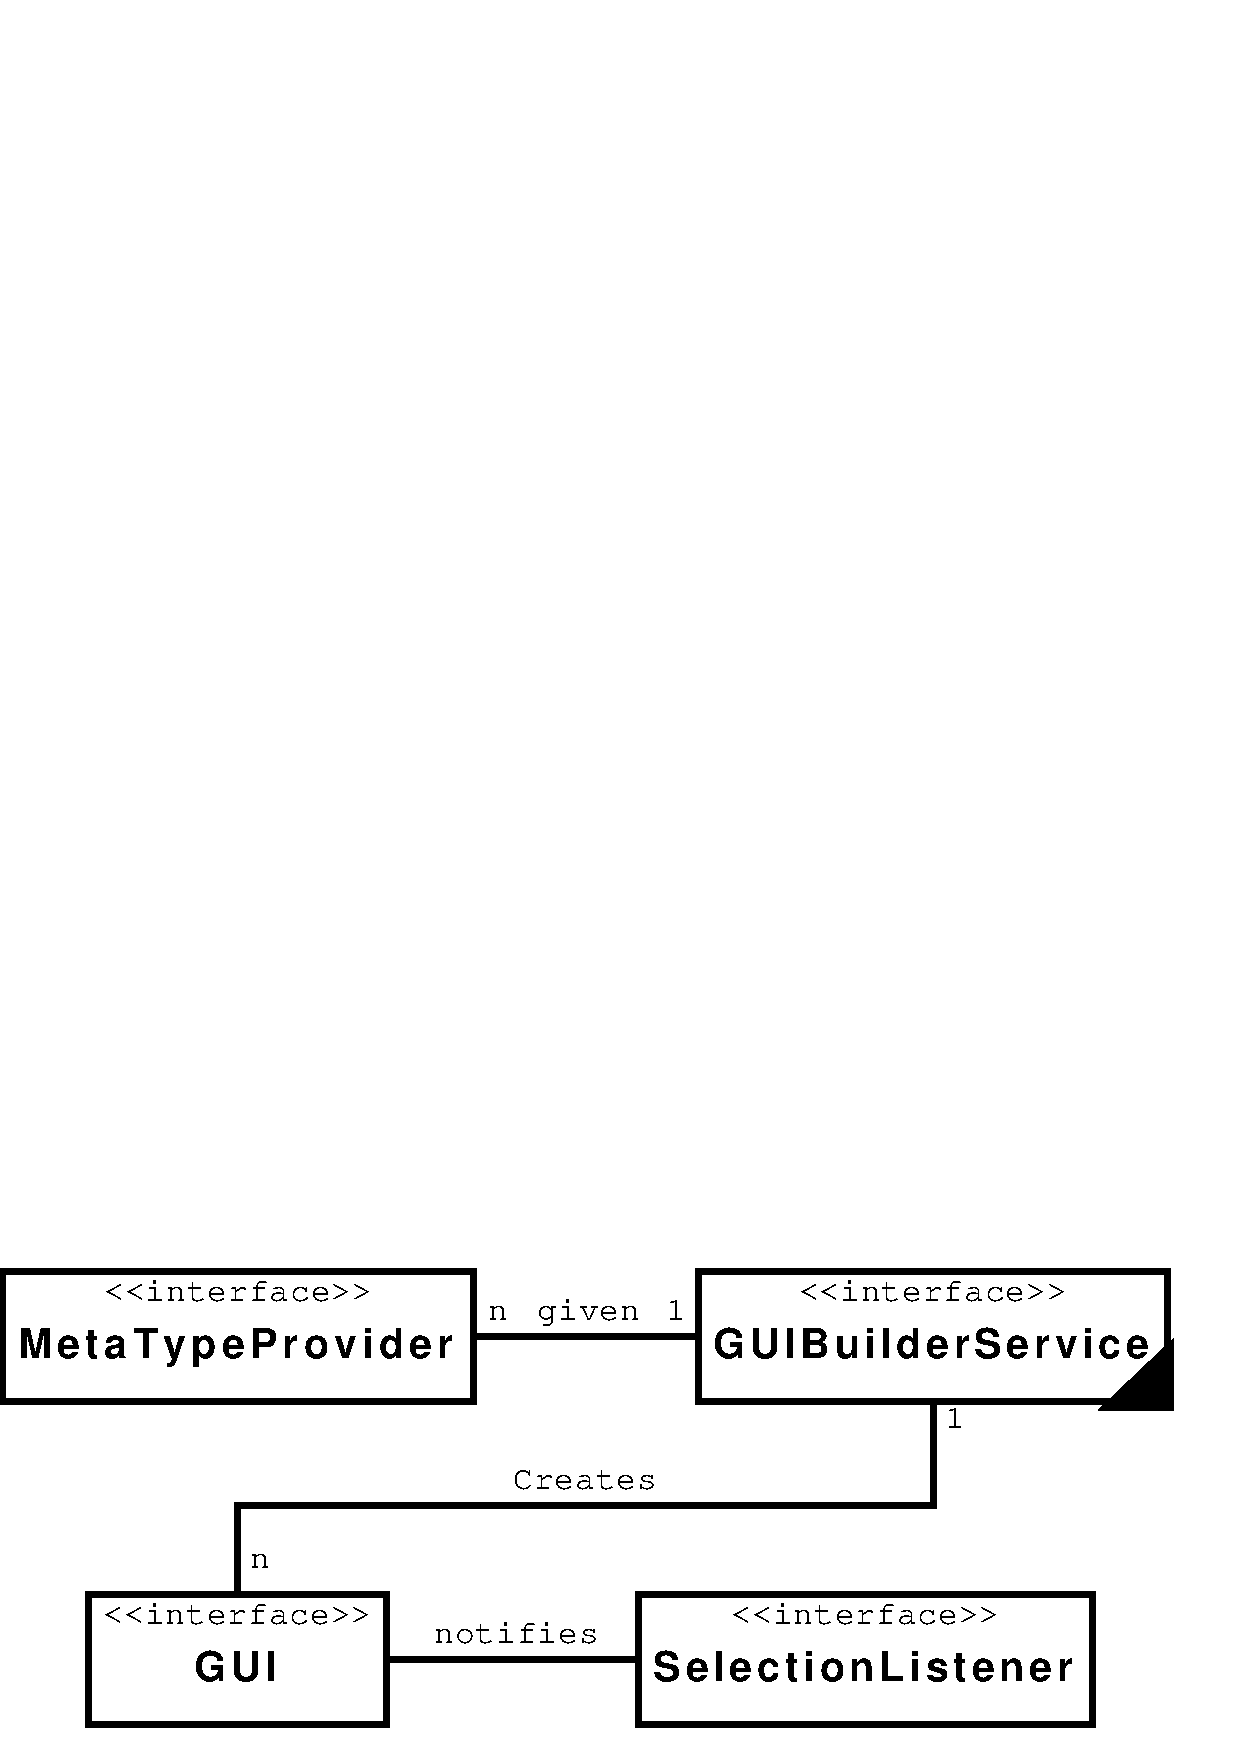
\includegraphics[width=90mm]{../img/guiCreationWorkflow.pdf}
\caption{GUI Creation Workflow}
\label{fig:guiCreationWorkflow}
\end{figure}

\orgcishellserviceguibuilder{}
